Geometry editor is used to define geometries of the user defined Petri net. The places within petri net have geometries which define each places graphical shape in simulation. The shapes can be either lines or coordinate locations, which are called as input points. These shapes are created and edited in the geometry editor.
To use geometry editor in Eclipse, first thing needed to do is to create a geometry and geometry diagram. To create them, a new General Project should be created by $General->Project$ which is found in $File->New->Project$, if it hasn't been made already. Give the project some name and click finish. 
Right click the project folder $New->Other$. Find Geometry diagram from the list, the search functionality might help, choose it and click next. Refer to Figure~\ref{fig:ge-wiz-select}. Name it, click next, name the geometry and then click finish. On the project explorer leaf two new files have now been generated, geometry and geometry diagram. The geometry diagram is Graphical geometry editor and the geometry is the model, presented in a tree view, that geometry diagram edits. Editing geometry within the tree view of the geometry will not do correct changes on the graphical view of the geometry. If the geometry diagram is not open, open it now.

\begin{figure}[htp]
\begin{center}
  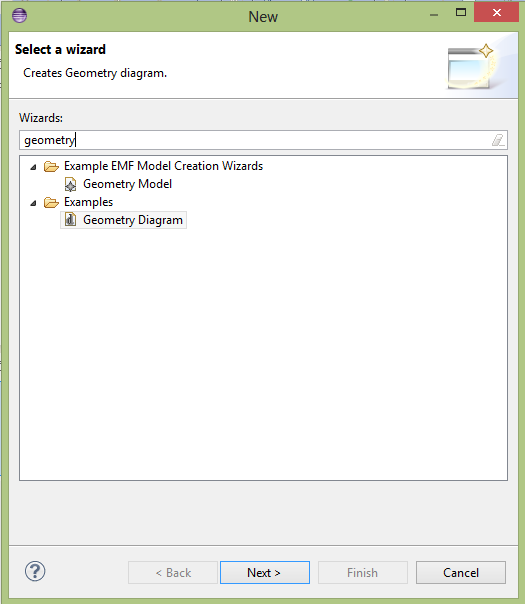
\includegraphics[width=0.8\textwidth]{image/ge-wiz-select.png}
  \caption{Select wizard for Eclipse plugins. The search functionality has been used to find geometry diagram.}
  \label{fig:ge-wiz-select}
\end{center}
\end{figure}

Figure~\ref{fig:ge-diag-empty} presents empty graphical geometry editor view. Right hand side of the view has tool palette, which has all the available tools to be used. Rest of the view is taken by the canvas. On the geometry palette clicking Input point, or connector allows user to create different points on the canvas. These points can be also created by hovering mouse on canvas and a selector tool appears after a while. Input point and connector are described there by the symbols seen in geometry palette. Line tool allows drawing connections between connectors with each other. Line can also be created by hovering mouse over a connector, which presents arrows. By clicking and dragging the arrow the new line can be thus created. Bend points are generated by clicking a point within a line and then by dragging said point. 

\begin{figure}[htp]
\begin{center}
  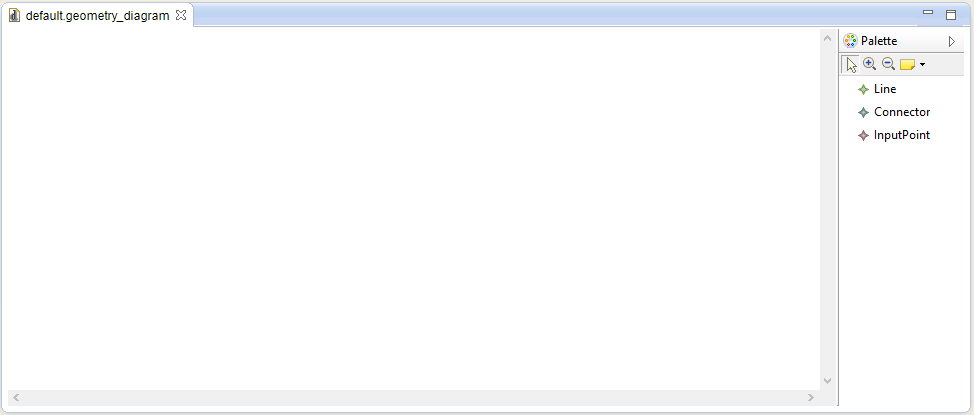
\includegraphics[width=0.8\textwidth]{image/ge-diag-empty.png}
  \caption{View of graphical geometry editor. Geometry palette can be seen on the right hand of the view and the rest is taken by canvas.}
  \label{fig:ge-diag-empty}
\end{center}
\end{figure}

Picture Figure~\ref{fig:ge-diag-exam} illustrates one example created with graphical geometry editor. Input points are presented by circles and connectors are represented by squares. A geometry object line is presented by a line in the canvas. The Bend points of a line can be seen as filled squares. However, the bend points are only visible when the line is selected. The labels, appearance labels and token appearance labels are visible in the canvas next to their graphical visualization on the canvas. The labels have prescript in the same order, called Label, Visual and Token. The labels are used to connect geometry objects to petri net and to their 3D visualization.

\begin{figure}[htp]
\begin{center}
  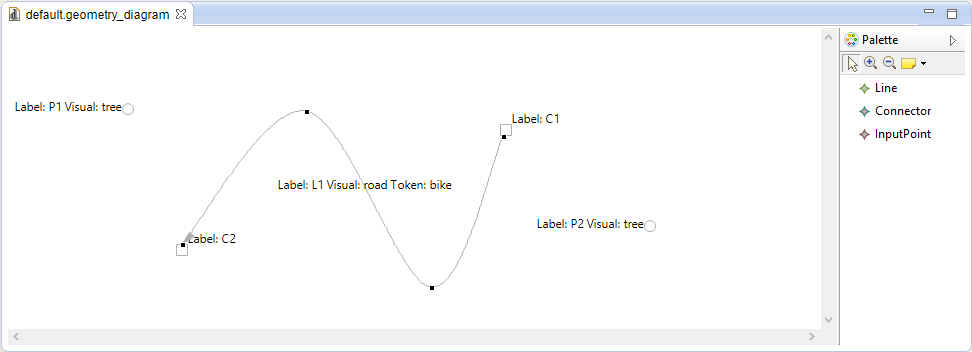
\includegraphics[width=0.8\textwidth]{image/ge-diag-exam.png}
  \caption{View of graphical geometry editor with different geometry objects.}
  \label{fig:ge-diag-exam}
\end{center}
\end{figure}

By clicking some geometry object, a property view of said object opens. If this is not visible right click on a geometry object within the canvas and click Show Properties View to open property view.
The properties view of input point as seen in Figure~\ref{fig:ge-prop-input} has following properties available for editing: Appearance Label, Label, XLocation and YLocation. Appearance Label denotes the appearance, such as a tree, a traffic light, a planet, etc, of the input point within the 3d simulator. Appearance label has to have some labeling in it. Label is the name used in referring the input point within the software. All the geometry objects must have different names so that references don't lead to multiple objects. XLocation and Ylocation describe coordinate location of the input point. However, editing them will not change the location input point in the canvas.

\begin{figure}[htp]
\begin{center}
  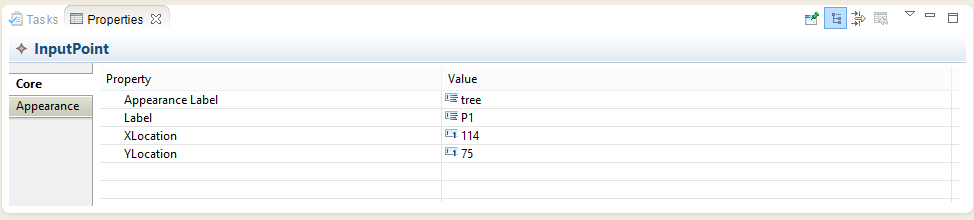
\includegraphics[width=0.8\textwidth]{image/ge-prop-input.png}
  \caption{Properties view of input point geometry object.}
  \label{fig:ge-prop-input}
\end{center}
\end{figure}

The properties view of Connector as seen in Figure~\ref{fig:ge-prop-conn} has following properties available for editing: In, Label, Out, XLocation and YLocation. In refers to the lines that go to the connector. And Out refers to the lines that go from the connector. Label is the name used in referring the Connector within the software. All the geometry objects must have different names so that references don't lead to multiple objects. XLocation and Ylocation describe coordinate location of the connector. However, editing them will not change the location connector in the canvas.

\begin{figure}[htp]
\begin{center}
  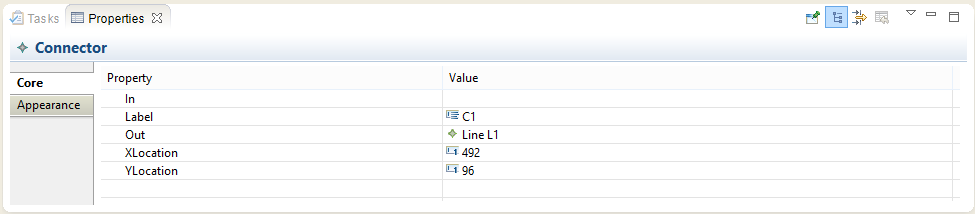
\includegraphics[width=0.8\textwidth]{image/ge-prop-conn.png}
  \caption{Properties view of connector geometry object.}
  \label{fig:ge-prop-conn}
\end{center}
\end{figure}

The properties view of Line as seen in Figure~\ref{fig:ge-prop-line} has following properties available for editing: Appearance Label, Begin, End, and Label. Appearance Label denotes to the appearance, such as a cable, a track, empty space, etc, of the line within 3d simulator. The appearance will extrapolated over the curve of the line, thus creating continuous shape. Begin and End denotes the connector of the line, which is the starting and ending point respectively of the parametric curve that is line geometry. Label is the name used in referring the line within the software. All the geometry objects must have different names so that references don't lead to multiple objects.

\begin{figure}[htp]
\begin{center}
  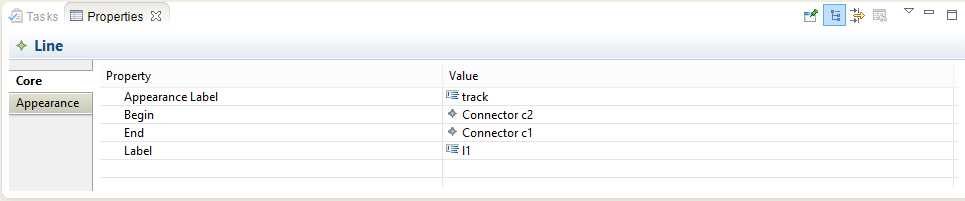
\includegraphics[width=0.8\textwidth]{image/ge-prop-line.png}
  \caption{Properties view of line geometry object.}
  \label{fig:ge-prop-line}
\end{center}
\end{figure}

To validate that the geometry doesn't have any duplicate Labels, the geometry should be opened in the tree view. Right click on the tree view window and choose the Validate option. If there are duplicate labels, an error message will pop up. The tree view of the geometry used as an example in this part of handbook can be seen in Figure~\ref{fig:ge-tree-exam}

\begin{figure}[htp]
\begin{center}
  \includegraphics[width=0.8\textwidth]{image/ge-tree-exam.png}
  \caption{Tree view of the geometry.}
  \label{fig:ge-tree-exam}
\end{center}
\end{figure}

